%======================================================================
\subsection{BW-PDM-11 --- Plan: the vault material library (24 Oct 2026, for approval)}\label{sec:pdm11-plan}
%======================================================================

You asked on 24 Oct whether there is an open-source material database we can use, and then: ``yes, plan the vault
material library''. What you want is a \emph{shop} library stored in the vault: the materials you actually buy
(6061-T6 plate, 1045/C45 bar, PETG, POM-C, \ldots), with values from the supplier's datasheet, shared by every part of
the vault, and revised and approved like the rest of the vault's data. This plan covers where those materials live,
how FreeCAD finds them, how a released part keeps the values it was released with, the trap of appearance-only
``materials'', units, stock forms and price, a supplier CSV import, and how Claude adds materials. Nothing is built yet.
It builds on the folder vault (\eref{PDM-04}), the lifecycle (\eref{PDM-05}), the part properties
(\S\ref{sec:partprops}) and Vault Settings (\eref{PDM-09}, \eref{DRW-01}).

\paragraph{The short answer to your question.} Yes: FreeCAD 1.x ships one, and BruceWorx already uses it. Its
\emph{Standard} folder has 125 engineering materials, every one with a density, most with strength and elastic values
(93 steels under EN names, 6 aluminium alloys including 6061-T6 and 7075-T6, 13 thermoplastics, glass, concrete,
wood). It is a good \emph{starting point} but not a shop library: it has no PETG, no ``1045'' by that name (it has
\code{Steel-1C45} and \code{C45E}), no stock sizes and no prices, and its values are typical handbook values, not your
supplier's. Its licences are mixed, not all LGPL: of the 125 Standard cards 95 are LGPL-2.0-or-later, 18 CC-BY-3.0,
4 CC-BY-SA-4.0, 2 CC-BY-4.0 and 1 GPL; the Appearance folder is GPL, the Machining folder CC-BY-3.0. Copying a card
into the vault therefore keeps its author and licence lines (attribution). Web databases such as MatWeb are free to
read, but their terms do not allow bulk copying \verify; the plan uses them, and supplier sheets, one material at a
time, typed in or imported from a CSV, never scraped.

%----------------------------------------------------------------------
\subsubsection*{1. What the spikes showed (24 Oct)}

Four scripts ran in \code{FreeCADCmd} 1.1.4 on a copy of your configuration, through the FreeCAD slot limiter, with
every library and part in a scratch folder (\file{materials-plan/spike\_materials.py}, \file{spike\_missing.py},
\file{spike\_extra.py}, \file{spike\_units.py}). Your vault and your User material folder were not touched.

\begin{center}
\small
\begin{tabularx}{\linewidth}{@{}>{\hsize=0.8\hsize}X>{\hsize=1.2\hsize}X@{}}
\toprule
Library: check & Result\\
\midrule
Libraries FreeCAD loads & \emph{System} (\file{share/Mod/Material/Resources/Materials}, 200 cards), \emph{BruceWorx}
  (\file{Mod/BruceWorx/Materials}, 11 electronics cards, registered as a workbench library at start-up), \emph{User}
  (empty); 211 materials, listed in 1\,ms\\
Census by folder (cards / with density) & Standard 125/125, Fluid 6/6, BruceWorx 11/8, Machining 13/0 (cutting data
  only), Appearance 23/0, Patterns 32/0\\
The trap & Appearance \code{Steel} has \emph{no physical model} at all. Assigned to a 10\,mm cube: \code{MaterialName}
  reads ``Steel'', \code{Mass} 0.0\,kg. FreeCAD's own \emph{Set Material} dialog hides such cards (its filter
  requires a physical model); a script choosing by name does not, which is how it reached a part today\\
A density filter & \code{MaterialFilter} with \code{RequiredModels = [Density]}: 139 cards (Standard, Fluid,
  BruceWorx)\\
The name shown & always the \emph{file name}: a card \file{PETG.FCMat} whose \code{General/Name} says ``PETG
  (Prusament)'' shows as ``PETG'' (\file{MaterialLoader.cpp}: ``Always get the name from the filename'')\\
Registering a folder at run time & a group \code{Mod/Material/Resources/Modules/<name>} with \code{ModuleDir}; the
  materials appear after \code{MaterialManager().refresh()} (0.03\,s), not before\\
Unregistering & empty \code{ModuleDir} or remove the group, then refresh: the library leaves the list, but its
  materials \emph{stay findable by UUID until FreeCAD restarts} (a static cache, \code{\_materialEntryMap}, is never
  cleared: an upstream bug)\\
A card edited, then refresh & the new values are used: a part reopened went from 0.1355 to 0.1400\,kg when the card's
  density went from 2710 to 2800\,kg/m$^3$. The part \emph{follows} the library\\
Same UUID in two libraries & one wins, by load order and that cache (here the copy won). Never register two cards with
  one UUID\\
\bottomrule
\end{tabularx}
\end{center}

\begin{center}
\small
\begin{tabularx}{\linewidth}{@{}>{\hsize=0.8\hsize}X>{\hsize=1.2\hsize}X@{}}
\toprule
Part and card: check & Result\\
\midrule
What a part file stores & \code{<PropertyMaterial uuid="6a1e\ldots6061"/>} and nothing else: no name, no density
  (``2710'' appears nowhere in \file{Document.xml})\\
Opened where the library is not registered & ``Invalid Document.xml: Material not found'' in the report view; the body
  falls back to \emph{Default}; \code{Mass} 0\,kg, \code{MaterialName} empty\\
\quad then saved there & the \emph{Default} UUID is written. Reopened with the library back: still Default. \textbf{The
  material is lost for good, silently}\\
A vault card that inherits & \code{Inherits: Aluminum 6061-T6} (the Standard card's UUID) and overrides the density:
  the card gets the parent's thermal values and product URL too. A missing parent is ignored without a message\\
Extra data in a card & a top-level \code{BruceWorx:} block (code, revision, stock list) is ignored by FreeCAD, so vault
  data can travel inside the card; an unknown property inside a model (\code{StockThickness}) is dropped silently;
  \code{Tags} are read\\
Bad values & \code{Density: "heavy"} loads without a word; \code{partprops} then gives no mass. Nothing validates cards\\
Saving through the API & \code{MaterialManager.save(library, material, path, overwrite=True)} into a library that is not
  read-only: works; the file starts with a byte-order mark and a ``File created by FreeCAD'' comment, the density is
  rewritten in kg/m$^3$\\
Costs model & \code{ProductURL}, \code{Vendor}, \code{SpecificPrice} (a float, ``currency per mass'', no currency);
  7.80 reads back as 7.800000190734863 (single precision)\\
Units a supplier sheet uses & parse: \code{35 ksi} = 241.3\,MPa, \code{42000 psi}, \code{1.27 g/cm\^{}3},
  \code{0.098 lb/in\^{}3} = 2712.6\,kg/m$^3$, \code{490 lb/ft\^{}3}, \code{1/2 in}; do \emph{not} parse:
  \code{g/cm3}, \code{kg/m3}, \code{g/cc}, \code{Msi}, \code{\O 12.7}\\
External material interface & exists upstream (a Python class serving materials), but \code{BUILD\_MATERIAL\_EXTERNAL}
  is OFF in our build and the interface is experimental\\
\bottomrule
\end{tabularx}
\end{center}

\paragraph{What BruceWorx does with materials today.} \code{MaterialName} (BOM column, title block, required at submit)
is computed from the bodies' \code{ShapeMaterial.Name}, and \code{Mass} is volume times density
(\code{partprops.computed\_mass}, \code{\_density\_kg\_per\_mm3}; an appearance-only card already gives ``no mass'' instead
of a failed save). The right panel's \emph{Material} field opens FreeCAD's \code{Std\_SetMaterial}. The Create Vault wizard
offers a free-text company property \code{MaterialSpec} (``ASTM B221 6061-T6''), and a sheet-metal rule copies its
material text into it. The bridge has no material tool: Claude sets \code{ShapeMaterial} through \code{run\_python}. One
precedent matters: the sheet-metal rules (\eref{MOD-06}) are copied into the part's VarSet ``so the rules a part takes
stay as they were when it took them''. Materials need the same, for the same reason.

\paragraph{Three findings to act on.} (1) A FreeCAD part names its material by UUID only, so a part opened anywhere
the library is missing shows Default and 0\,kg, and \emph{saving it there loses the material}; the part file must carry
its own copy. (2) Editing a card changes every part that uses it, released or not, so a released part needs pinned
values. (3) Every place BruceWorx (or Claude) picks a material must refuse cards without a density.

%----------------------------------------------------------------------
\subsubsection*{2. Theory}

\paragraph{A material is an item; its values are a revision.} The vault already separates what a thing \emph{is} from
what it \emph{says} at a moment: an \emph{Item} has a permanent P/N, its \emph{Revisions} carry the state, and each
revision points at a content-addressed file version (figure~\ref{fig:pdm-model}). A material fits the same shape
(figure~\ref{fig:pdm11-model}). The \emph{material} (``6061-T6 plate'', code \code{MAT-0001}) is permanent and keeps one
FreeCAD UUID for life, so a part's reference never breaks. A \emph{material revision} (01, 02, \ldots\ before release; A,
B, \ldots\ after, as for parts) holds the engineering values: density, strengths, modulus, the basis of those numbers and
the datasheet they came from. Its card is stored once, as an object named by its SHA-256, like any file version.
Price and stock sizes are \emph{commercial} data: they change every quarter without changing a single mass or stress, so
they sit beside the revision, editable, with their history in the journal, and never trigger a re-approval.

\begin{figure}[!htbp]
\centering
\begin{tikzpicture}[>=Stealth,
  ent/.style={draw=bwblue!70,fill=bwblue!5,rounded corners=2pt,align=left,font=\scriptsize,inner sep=4pt,text width=3.9cm},
  com/.style={ent,draw=bworange!80,fill=bworange!6},
  prt/.style={ent,draw=bwgreen!80,fill=bwgreen!6},
  rel/.style={font=\tiny\color{bwgrey},align=center}]
\node[ent] (mat) at (0,0) {\textbf{Material}\\code \code{MAT-0001} (permanent)\\FreeCAD UUID (permanent)\\name = card file name\\family (folder)};
\node[ent] (rev) at (5.3,0) {\textbf{Material revision}\\01, 02 \ldots\ A, B \ldots\\state WIP, Released, Obsolete\\density, yield, UTS, $E$, $\nu$\\basis, source (datasheet)};
\node[ent] (card) at (10.6,0) {\textbf{Card version}\\\file{.FCMat}, SHA-256\\values hash $h$\\written once in \file{objects/}};
\node[com] (stock) at (0,-2.8) {\textbf{Stock \& price}\\form, size, price/kg, currency\\supplier, supplier P/N\\not revisioned; history in journal};
\node[prt] (snap) at (5.3,-2.8) {\textbf{Material snapshot} (per body)\\UUID, code, revision, $h$\\name, density, \ldots\\saved in the part file};
\node[prt] (prev) at (10.6,-2.8) {\textbf{Part revision}\\check-in records\\\code{materials: \{uuid: (code, rev, $h$)\}}\\pinned at release};
\draw[->] (mat) -- node[rel,above]{has 1..*} (rev);
\draw[->] (rev) -- node[rel,above]{stored as} (card);
\draw[->] (mat) -- node[rel,right]{has 0..*} (stock);
\draw[->] (snap) -- node[rel,right,pos=0.4]{copy of} (rev);
\draw[->] (prev) -- node[rel,above]{pins} (snap);
\end{tikzpicture}
\caption{Material data model, drawn like the PDM model of figure~\ref{fig:pdm-model}. Blue is the library, orange the
commercial data that changes without approval, green what travels with a part.}
\label{fig:pdm11-model}
\end{figure}

\paragraph{Reference or snapshot? Both, for different jobs.} Let $L_t$ be the library at time $t$ and $m$ the material
of a part $p$ of volume $V$. With a pure reference the part's mass is
\[
  M(p,t) = V(p)\,\rho\bigl(L_t(m)\bigr),
\]
which moves whenever the library moves --- also for a released part, whose drawing and BOM printed the old number. Release
promises the opposite: everything derived at release is reproducible from the released data alone. So a part carries a
snapshot $s = (m, r, h, \rho, \ldots)$ of the revision $r$ it was given, and
\[
  M(p) =
  \begin{cases}
    V(p)\,\rho(s) & \text{if } p \text{ is released (pinned), or the library cannot resolve } m,\\
    V(p)\,\rho\bigl(L_t(m)\bigr) & \text{otherwise (WIP follows the latest released revision).}
  \end{cases}
\]
The values hash $h = \mathrm{SHA256}(\mathrm{canon}(r))$ is taken over the engineering values only, in SI, keys sorted,
numbers to 9 significant digits; a price change leaves it alone. Comparing $h(s)$ with the hash of the library's current
revision gives the ``material newer'' badge, exactly as \emph{newer version available} does for files. This is the same
rule \eref{PDM-06} applies to children: a WIP assembly takes the latest released child, a released one is pinned.

\paragraph{How much a density matters.} $\delta M / M = \delta\rho/\rho + \delta V/V$. The handbook 6061 density
(2700\,kg/m$^3$) and a supplier's 2710 differ by 0.37\,\%: invisible on one bracket, 3.7\,g on a 1\,kg assembly. The
strengths differ much more, and in the direction that matters: the handbook's \emph{typical} yield of 6061-T6 is 276\,MPa,
the plate specification's \emph{minimum} is 35\,ksi = 241\,MPa \verify, 13\,\% lower. Mass wants typical (nominal)
values; a strength check wants minimums. So every revision records its \emph{basis} (typical, minimum, measured), and
simulation (\eref{SIM-03}) refuses a typical yield for a safety factor unless told to.

\paragraph{Units.} Cards store SI, as FreeCAD does (the API returns kg/mm$^3$); the vault shows them in its units.
Conversions are exact definitions: 1\,lb/in$^3$ = $0.45359237 / 0.0254^3$ = 27\,679.9\,kg/m$^3$ (the spike's value), 1\,ksi =
6.894757\,MPa, 1\,\$/lb = 2.20462\,\$/kg. A supplier's ``specific gravity'' $SG$ becomes $\rho = 999.97\,SG$\,kg/m$^3$
(water at 4\,\textdegree C; $1000\,SG$ is within 0.003\,\%).

\paragraph{Price from stock, not from the finished part.} A part is cut from a blank, so its material cost is
\[
  C = c_{\mathrm{kg}}\;\rho\;V_{\mathrm{blank}},\qquad
  V_{\mathrm{blank}} = (L + 2a)(W + 2a)\,t_{\mathrm{stock}},\quad t_{\mathrm{stock}} = \min\{t \in T : t \ge H + a_z\},
\]
with $T$ the plate thicknesses you stock and $a$ the saw and machining allowance; for round bar
$V_{\mathrm{blank}} = \tfrac{\pi}{4} d^2 (L + k)$ with the smallest stocked $d \ge D + 2a$ and kerf $k$. Example: the
$100\times50\times10$\,mm bracket of figure~\ref{fig:pdm11-picker} (0.1355\,kg at 2710\,kg/m$^3$), cut from 12.7\,mm plate with
$a = 3$\,mm: blank $106\times56\times12.7$ = 75\,387\,mm$^3$ = 0.2043\,kg, \$1.59 at \$7.80/kg; buy-to-fly ratio
$0.2043/0.1355 = 1.51$. The \code{Stock} property that sheet metal already writes (``Sheet 16\,ga Al 5052'') becomes the
general home of the chosen stock.

%----------------------------------------------------------------------
\subsubsection*{3. Design}

\paragraph{Where the files live.} Four options were weighed:
\begin{center}
\small
\begin{tabularx}{\linewidth}{@{}>{\raggedright\arraybackslash}p{3.3cm}XX@{}}
\toprule
The library is \ldots & For & Against\\
\midrule
\textbf{a folder in the vault} \file{<vault>/materials/} (proposed) & travels with the vault to every Mac; Finder-readable;
  FreeCAD reads it as a library; the cards carry the vault block & files replaced in place (one writer at a time, like
  \file{drawing\_standards.json})\\
a local cache rebuilt from the journal & nothing in place in iCloud & invisible in Finder; a second copy to keep in
  step; harder to explain\\
FreeCAD's User library & no code & per Mac, not per vault; editable by FreeCAD's editor, so values change unseen\\
the external material interface & a real database & off in our build, experimental; a C++ build flag\\
\bottomrule
\end{tabularx}
\end{center}
Proposed layout, in the vault's style (the truth is the journal and the objects; \file{materials/} is what FreeCAD reads
and can be rebuilt from them by Check Vault):
\begin{lstlisting}
<vault>/
  materials/                       FreeCAD library while the vault is open
    Aluminium/6061-T6 plate.FCMat  current card; file name = name shown
    Steel/1045 - C45 bar.FCMat
    Plastic/PETG (Prusament).FCMat
  objects/ab/<sha256>.FCMat        every revision's card, written once
  journal/<actor>.jsonl            material_create, _revise, approve, ...
\end{lstlisting}
The current card is the latest \emph{released} revision; a WIP revision lives only in \file{objects/} and the journal until
it is approved (and, with \emph{Show WIP}, in the picker, read from the object). Each card is a normal FreeCAD card plus the
ignored \code{BruceWorx:} block (code, revision, state, values hash, basis, source, stock list), so a card copied out of the
vault still says where it came from. Names are unique within a family (two files cannot share a name in one folder).

\paragraph{Registering it while a vault is open.} The vault client's session listener (it already reacts when
\code{VaultPath} changes and at start-up) registers \code{Resources/Modules/Vault <name>} with
\code{ModuleDir = <vault>/materials}, \code{ModuleReadOnly = true} and the vault icon, asks the iCloud helper to download
any card not yet on this Mac (FreeCAD skips iCloud placeholders without a word), and calls \code{refresh()} (0.03\,s). On
close it empties \code{ModuleDir}, removes the group and refreshes: the library leaves the picker. Its materials stay
resolvable until FreeCAD quits (the upstream cache), which is harmless, since UUIDs are unique; question~10 asks whether to
fix the cache. At start-up a leftover \code{Vault *} group from a crash is removed unless it is the open vault's. The
library is read-only to FreeCAD, so its own material editor cannot change a vault card; \emph{Save as} there makes a copy
with a new UUID in the User library.

\paragraph{The part carries its material (the safety net).} When a body gets a material (picker, FreeCAD's dialog, a
script, the bridge: the \code{partprops} observer already watches \code{ShapeMaterial}), BruceWorx writes a hidden map
\code{BW\_MaterialSnapshot} on the body: UUID, code, revision, hash, name, library, density and the other engineering
values. On opening a document:
\begin{enumerate}[nosep]
  \item body shows Default, snapshot names a material that \emph{resolves now} (library registered later): put it back;
  \item it does \emph{not} resolve: keep the snapshot, compute \code{Mass} and \code{MaterialName} from it, and show the
        notice of figure~\ref{fig:pdm11-picker} (right). Saving keeps the snapshot, so nothing is lost; when the vault is
        opened, the material is put back;
  \item the snapshot's hash differs from the library's current revision: WIP parts take the new revision at the next open
        (a toast with the mass change); released parts keep theirs and show \emph{material rev B available}.
\end{enumerate}
The observer must never write 0\,kg or an empty \code{MaterialName} over a part only because its library is missing (it
would today). The part gets two visible properties beside \code{MaterialName}: \code{MaterialCode} and
\code{MaterialRevision} (BOM columns, title block).

\begin{figure}[!htbp]
\centering
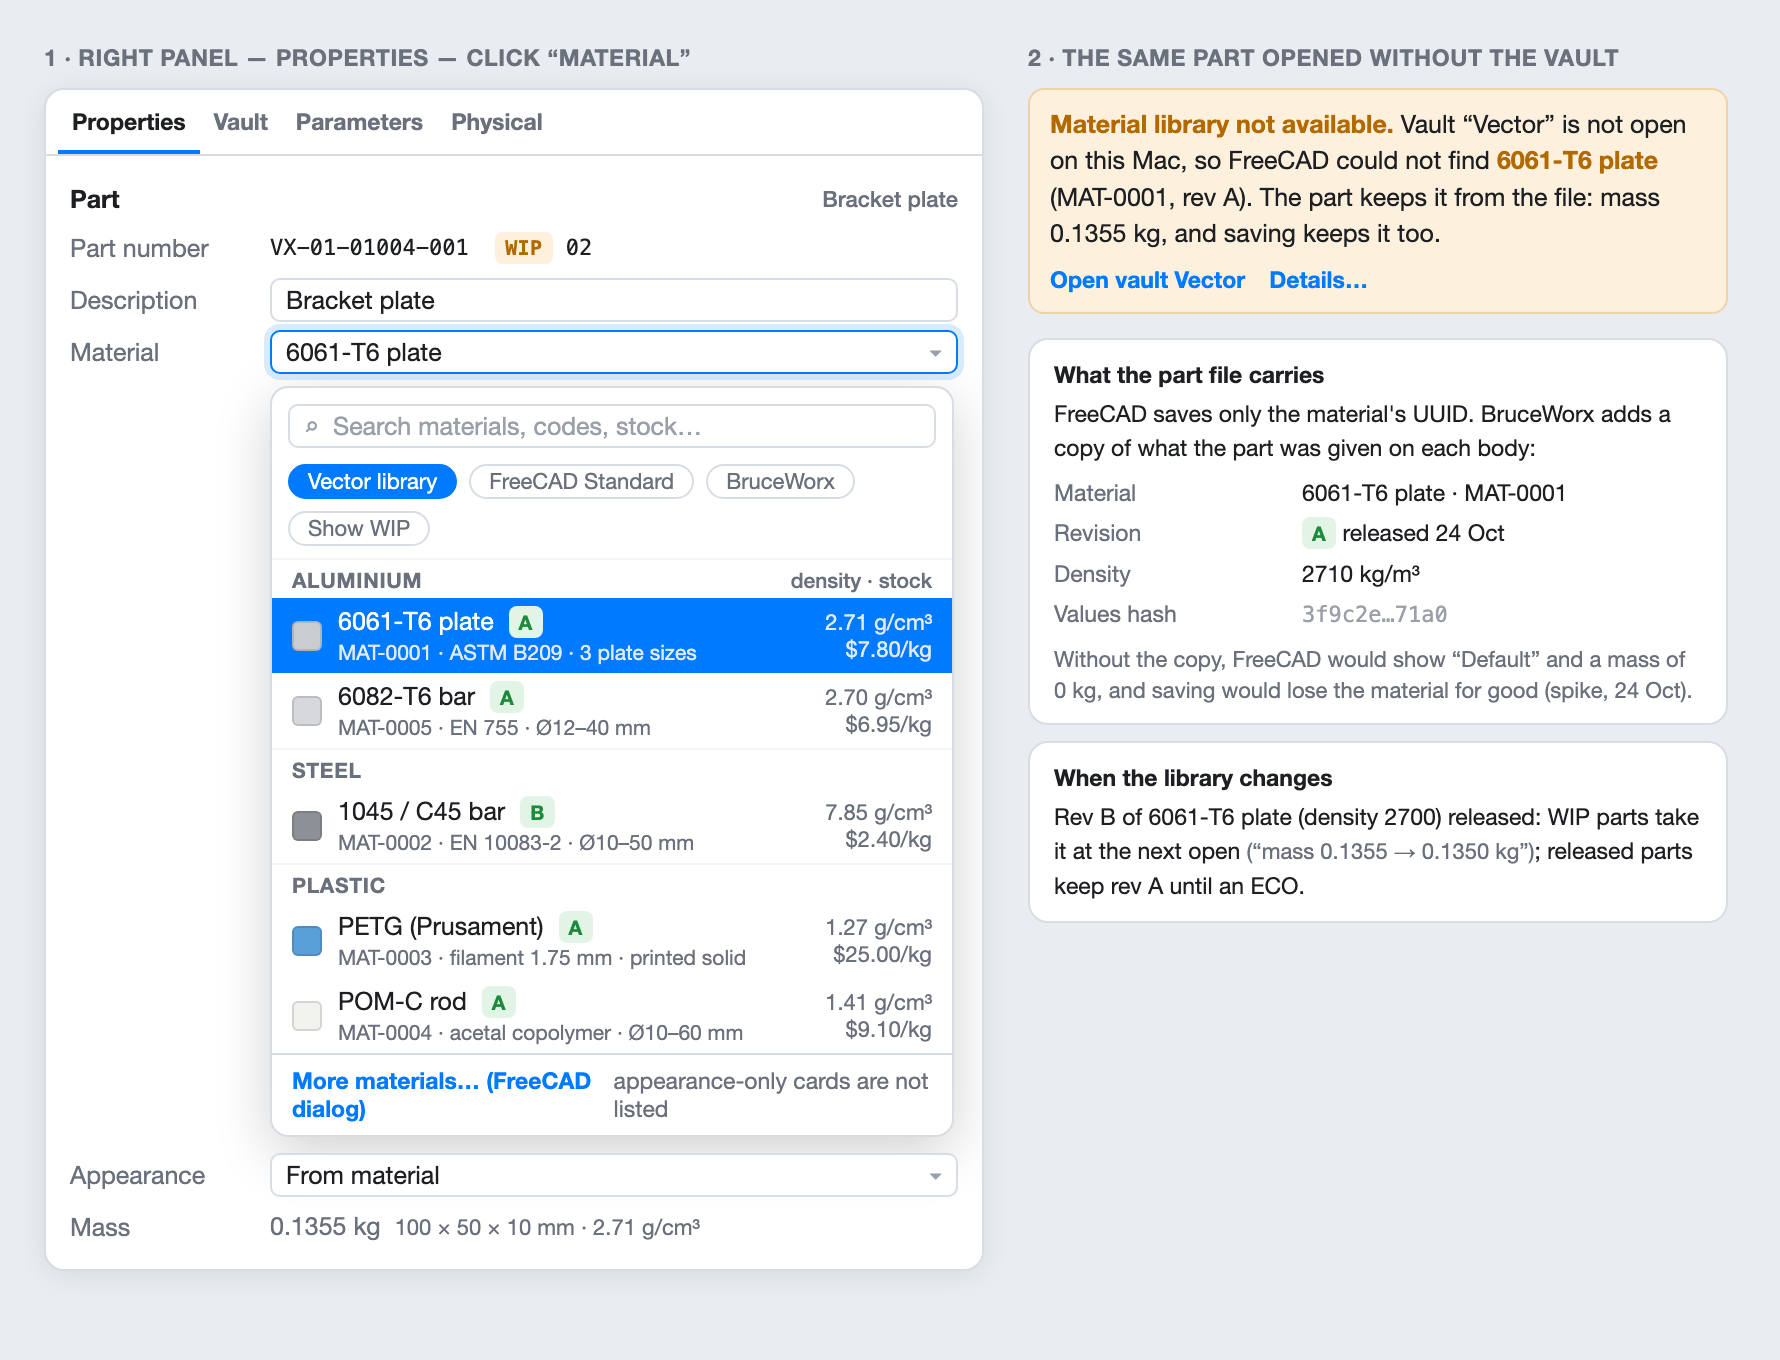
\includegraphics[width=\linewidth]{fig/pdm11_picker.png}
\caption{Mock: the right panel's \emph{Material} field opens the vault's picker (left): released vault materials by family,
with density and price per kg in the vault's units, filter chips for FreeCAD's Standard and BruceWorx libraries, and
FreeCAD's own dialog one click away. Cards without a density are never listed. Right: the same part opened on a Mac where
the vault is not open.}
\label{fig:pdm11-picker}
\end{figure}

\paragraph{Picking a material.} The \emph{Material} field opens a BruceWorx picker in place of \code{Std\_SetMaterial}
(figure~\ref{fig:pdm11-picker}): the open vault's released materials first, grouped by family, each with code, revision,
standard, density and price in the vault's units; chips add FreeCAD Standard, BruceWorx (electronics) or the vault's WIP
materials; search covers names, codes and stock sizes. It sets the material on every body of the part (or the selected
body), writes the snapshot, and fills \code{MaterialSpec} when the vault has that property and it is empty, as a sheet-metal
rule does. Every BruceWorx path that sets a material (picker, bridge, CSV, the KiCad board) uses one function,
\code{materials.assign}, which refuses a card without a density with a plain sentence (``Steel in the Appearance library
is a colour, not a material: use Appearance''). FreeCAD's own dialog already hides such cards.

\paragraph{Approval and revisions.} A new material starts as WIP revision 01; it can be used in WIP parts at once (a WIP
pill in the picker). \emph{Approve} (an approver, with a note and the datasheet attached as a vault attachment) releases
rev A; \emph{New revision} opens rev B as WIP; approving B makes it current, A is superseded; \emph{Retire} (with a reason
and where-used) hides it from the picker, and the Start page's vault health lists parts still using it. No ECR/ECO for a
material: the parts it touches are protected by the snapshot, and a released part changes only through its own ECO
(question~3). A part's check-in records its \code{materials} map; release pins it; the release checklist gains two lines,
``materials released'' and ``materials from the vault library'' (waivable, question~6). \emph{Where used\ldots} on a
material is read from those check-ins.

\paragraph{Stock forms and price.} Each material lists its stock: form (plate, sheet, round bar, square or flat bar, tube,
filament, block), size (thickness, diameter, $w\times h$, OD $\times$ wall, filament diameter), price per kg or lb with
currency, supplier and supplier P/N, minimum order. They live in the card's \code{BruceWorx:} block, not in FreeCAD's Costs
model (one price, no currency, single precision). In a later step the picker proposes the stock for the part
(section~2) and the BOM gains \code{StockMass} and \code{MaterialCost} columns (question~11).

\begin{figure}[!htbp]
\centering
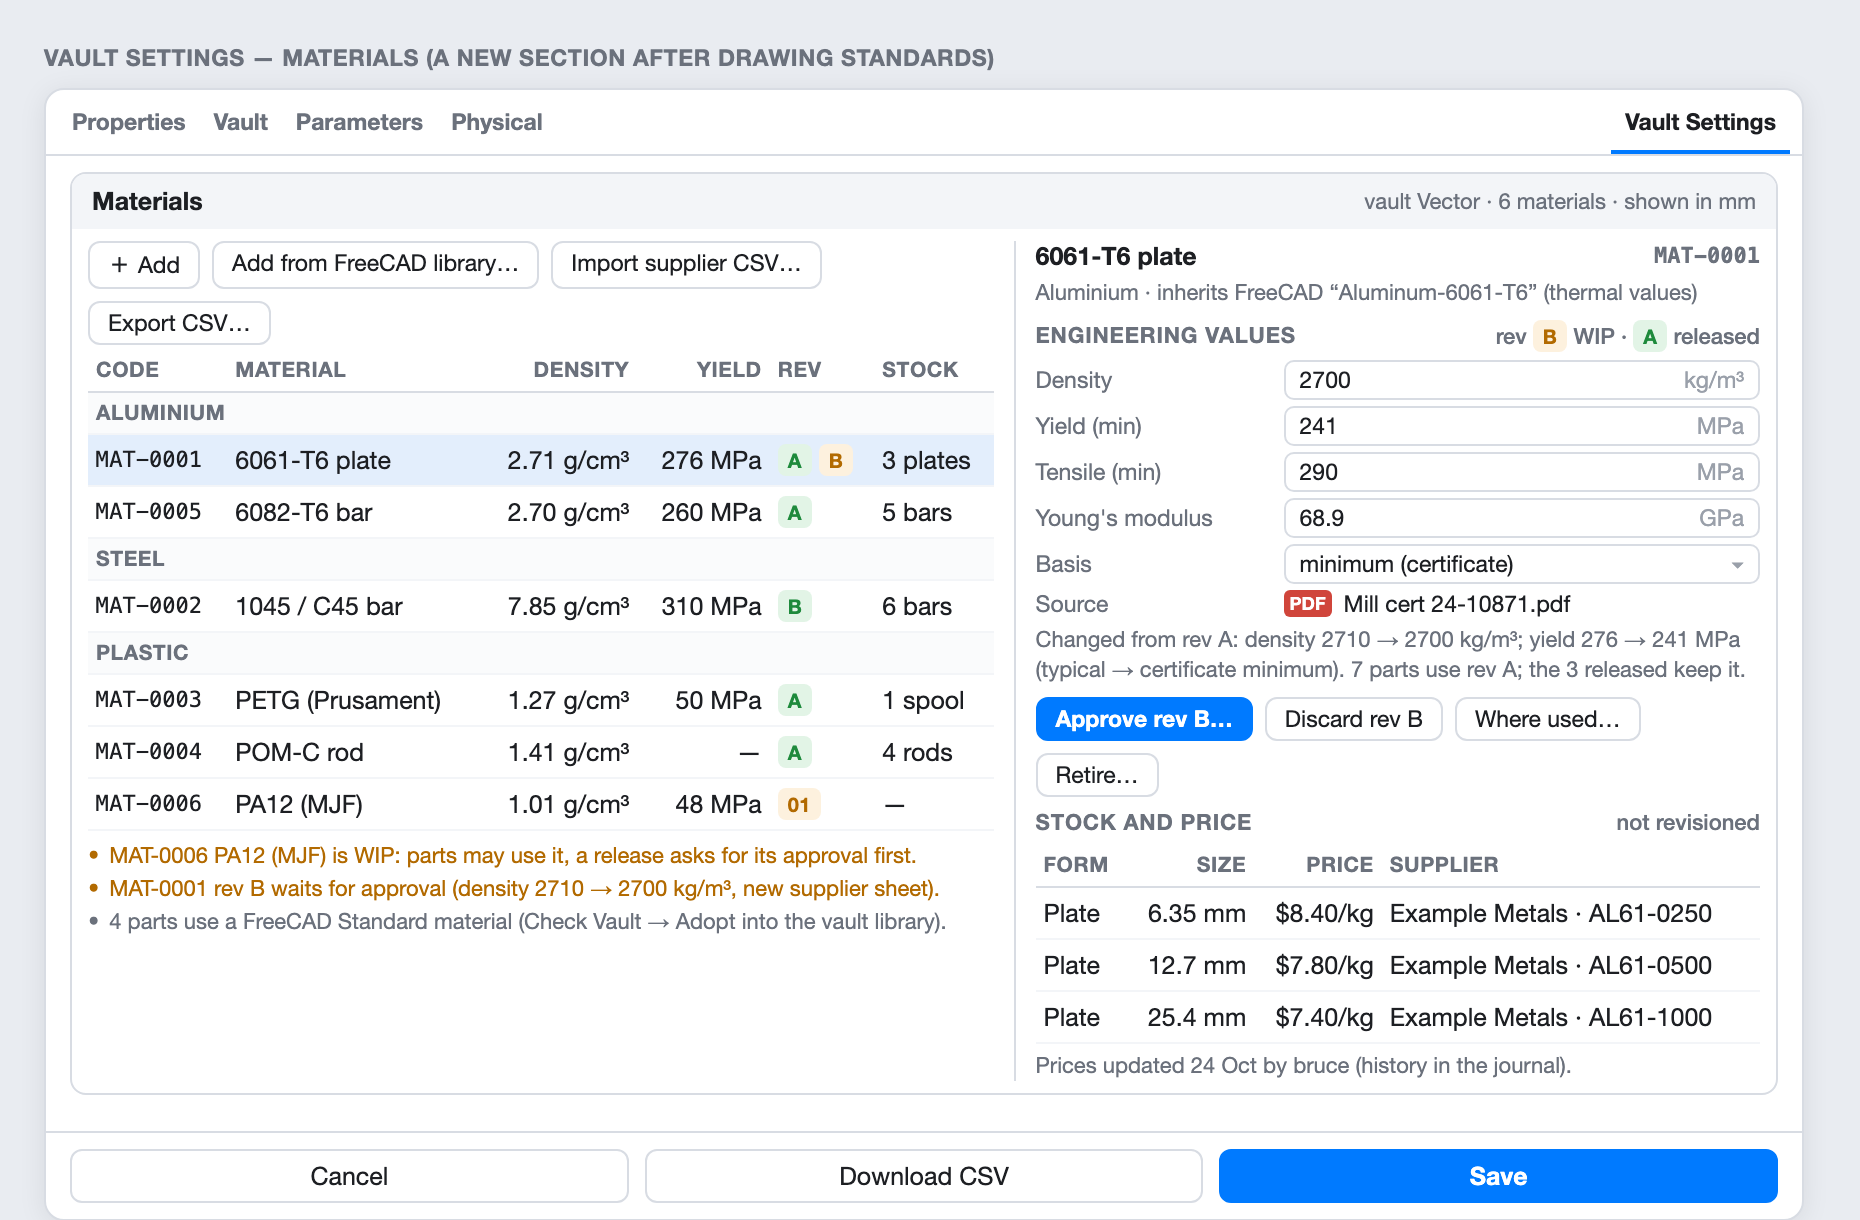
\includegraphics[width=\linewidth]{fig/pdm11_settings.png}
\caption{Mock: Vault Settings gains a \emph{Materials} section after Drawing standards. Left: the materials by family with
density, yield, revisions and stock count, and what needs attention. Right: the selected material: engineering values of
the WIP revision B with their basis and source, the change from rev A and its reach, Approve; below, stock and price, which
are edited without a revision.}
\label{fig:pdm11-settings}
\end{figure}

\paragraph{Vault Settings and the Start page.} Vault Settings gets a \emph{Materials} box (figure~\ref{fig:pdm11-settings};
the editor lives in its own module, as the drawing standards' does). \emph{Add} starts a blank WIP material; \emph{Add from
FreeCAD library\ldots} copies a Standard card as a new WIP material with a \emph{new} UUID, inheriting the original (so it
keeps the thermal data) and keeping its author and licence; \emph{Import supplier CSV\ldots} is below. Values are entered
and shown in the vault's units. The Start page's vault dashboard (\eref{PDM-10}) shows ``Materials: 5 released, 1 waiting
for approval'' in the vault's header and a health line for retired or non-vault materials in use; \emph{Check Vault} gains
\emph{Rebuild material library} and \emph{Adopt into the vault library} (maps Standard materials in vault parts to vault
materials, one check-out per part).

\paragraph{Importing a supplier sheet.} A materials CSV has its own columns (the vault-settings CSV has fixed ones):
\code{code, name, family, density, yield, uts, modulus, poisson, hardness, basis, source, inherits, form, size, price,
currency, per, supplier, supplier\_pn}; one row per stock line, rows with the same name merged into one material. Values
carry units per cell (``2.71 g/cm3'', ``35 ksi'') or take them from a units row. Header synonyms are matched (``Specific
gravity'' $\rightarrow$ density $\times$ 999.97, ``Tensile Strength, Yield'' $\rightarrow$ yield) and unit spellings FreeCAD
cannot parse are normalised first (\code{cm3}, \code{m3}, \code{g/cc}, \code{Msi}; the spike lists them). A preview shows
each row as \emph{new}, \emph{new revision} (with the changed values) or \emph{stock only}, with errors in red;
nothing is approved by an import. \emph{Export CSV} writes the same format.

\paragraph{Claude and other agents.} Through the same FreeCAD-free engine: bridge tools \code{vault\_materials} (read: list
and search, values in the vault's units), \code{set\_material} (model: by code or name, through \code{materials.assign}, so
appearance-only cards and cards without density are refused), and \code{vault\_material\_propose} (vault write: a WIP
material or revision with its source URL or attachment). There is deliberately no approve tool: approval stays a person's.
The CLI gets \code{bw-hooks vault material list | show | add | import-csv | where-used}. The bridge's
\code{get\_properties} already reports a missing material; it will report the snapshot too.

%----------------------------------------------------------------------
\subsubsection*{4. Build order and effort}

\begin{center}
\small
\begin{tabularx}{\linewidth}{@{}lXl@{}}
\toprule
\# & Step & Effort\\
\midrule
1 & Engine \file{bruceworx/materials.py} (FreeCAD-free): card read and write (no byte-order mark), the \code{BruceWorx:}
  block, values hash, unit normalising, journal operations in \file{pdm\_folder.py}, contract tests; OpenAPI & 1.5\,d\\
2 & Registration on vault open and close, iCloud download, start-up clean-up; the guard ``never two cards with one UUID'' & 0.5\,d\\
3 & Part side: \code{BW\_MaterialSnapshot}, restore guard, mass and name from the snapshot, \code{MaterialCode} and
  \code{MaterialRevision}, check-in \code{materials} map & 1.5\,d\\
4 & \code{materials.assign} and the picker on the right panel; the trap closed everywhere & 1.5\,d\\
5 & Vault Settings \emph{Materials}: list, editor, add from FreeCAD library, approve, new revision, retire, where-used & 2\,d\\
6 & Supplier CSV import and export with preview & 1\,d\\
7 & Bridge tools and CLI & 0.5\,d\\
8 & BOM, title block, release checklist lines, Start-page health, Check Vault (rebuild, adopt) & 1\,d\\
9 & Stock proposal, \code{StockMass} and \code{MaterialCost} in the BOM (may wait for \eref{MFG-04}) & 1\,d\\
10 & Acceptance on a scratch vault, then yours; write-up & 0.5\,d\\
\midrule
 & Total & 11\,d\\
\bottomrule
\end{tabularx}
\end{center}
Steps 1--4 alone fix today's two dangers (the silent loss and the appearance trap). \emph{Acceptance:} on a scratch vault, a
supplier CSV with 6061-T6 plate, 1045/C45 bar, PETG and POM-C becomes four materials, approved as rev A; a
$100\times50\times10$\,mm plate in 6061-T6 weighs 0.1355\,kg in the panel, the BOM and the title block; after the part is
released, rev B (2700\,kg/m$^3$) moves a WIP part to 0.1350\,kg and leaves the released one at 0.1355\,kg; the released part
opened and saved with no vault open still has its material and mass; Claude's \code{set\_material} refuses Appearance
\code{Steel}.

\paragraph{Risks.} \emph{Upstream cache}: materials of a closed vault stay findable until restart, and a deleted card too;
harmless with unique UUIDs, fixable in one line (question~10). \emph{Name = file name}: renaming a material renames its
file; the UUID stays, so parts are unaffected, but the old file must go in the same step or FreeCAD lists both (until
restart). \emph{iCloud}: a card not yet downloaded is invisible to FreeCAD; the download step and a health line cover it.
\emph{Two Macs editing settings at once}: \file{materials/} has the vault's one-writer rule; the journal still merges, and
Check Vault rebuilds the folder from it. \emph{Snapshot drift}: a body changed by FreeCAD's own dialog is caught by the
observer, which already watches \code{ShapeMaterial}. \emph{Printed parts}: PETG at 20\,\% infill weighs far less than
solid PETG; the library's value is the solid one, and a printed part needs \code{MassOverride} or a print profile
(question~12). \emph{Licences}: a copied Standard card keeps its CC-BY or CC-BY-SA lines; a vault's own cards are its
owner's.

%----------------------------------------------------------------------
\subsubsection*{Questions before PDM-11 starts}

\begin{enumerate}
  \item \textbf{Track and number.} A PDM epic, \eref{PDM-11}, in milestone M2 (the BOM, title block and release of
        \code{LE-02001} need right materials and masses)?\\
        \emph{Recommendation:} yes; simulation's material work (\eref{SIM-03}) builds on it later.
  \item \textbf{Where the library lives.} \file{<vault>/materials/}, one current card per material, registered while the
        vault is open, with every revision in \file{objects/} and the journal?\\
        \emph{Recommendation:} yes (the table in section~3).
  \item \textbf{Approval.} One approval by an approver, with a note and the datasheet attached, and no ECR/ECO for a
        material?\\
        \emph{Recommendation:} yes; released parts are protected by their snapshot and change only through their own ECO.
  \item \textbf{Reference and snapshot.} WIP parts follow the latest released revision; released parts keep the snapshot
        they were released with; every part file carries the snapshot?\\
        \emph{Recommendation:} yes; it is also what stops the silent loss found in the spike.
  \item \textbf{Price and stock outside revisions.} Edited freely (history in the journal), not part of the values hash?\\
        \emph{Recommendation:} yes; prices change too often to need an approval each time.
  \item \textbf{FreeCAD Standard materials in vault parts.} Allow them in WIP and warn at release (a waivable checklist
        line), or forbid them?\\
        \emph{Recommendation:} allow and warn; \emph{Adopt into the vault library} fixes them in one pass.
  \item \textbf{The appearance trap.} Never list or accept a card without a density anywhere BruceWorx or Claude sets a
        material?\\
        \emph{Recommendation:} yes; appearance stays under \emph{Appearance}.
  \item \textbf{Material codes.} \code{MAT-0001}, a counter of the vault's own, or a document type in the part-number
        scheme (\code{LE-09-\ldots})?\\
        \emph{Recommendation:} \code{MAT-0001}: materials belong to the company, not to a program.
  \item \textbf{Units in cards.} Always SI in the card, shown and typed in the vault's units?\\
        \emph{Recommendation:} yes; that is what FreeCAD expects and conversions are exact.
  \item \textbf{The upstream cache.} Add a one-line \code{[BW]} change that clears \code{\_materialEntryMap} on refresh, so
        closing a vault removes its materials at once?\\
        \emph{Recommendation:} yes, small and an upstream candidate; until then the behaviour is harmless.
  \item \textbf{Cost.} Stock and prices in the data now, and the stock proposal and BOM cost columns now (step~9) or with
        the release package (\eref{MFG-04})?\\
        \emph{Recommendation:} data now, cost columns with MFG-04.
  \item \textbf{Printed parts.} Leave the infill question to \code{MassOverride} for now, or add print profiles (effective
        density per material and infill)?\\
        \emph{Recommendation:} \code{MassOverride} now; print profiles with \eref{MFG-01}.
  \item \textbf{A starting set.} Seed a new vault with nothing, or offer a short list (6061-T6, 7075-T6, 1045/C45, 304,
        PLA, PETG, POM-C, PA6) copied from FreeCAD Standard as WIP?\\
        \emph{Recommendation:} offer the list in Create Vault, unticked by default; values marked ``typical'' until your
        supplier sheets replace them.
\end{enumerate}
